\documentclass[12pt,a4paper,oneside]{easysparc}

\usepackage{amsmath,amsfonts,mathdots,amssymb}
\usepackage{graphicx}
\usepackage{subcaption}
\usepackage{lipsum}
\usepackage{indentfirst}
\usepackage{makecell}
\usepackage{tabularx}
\usepackage{booktabs}
\usepackage{float}
\usepackage{algpseudocode, algorithm}
\usepackage{hyperref}
\usepackage{pdfpages}
\usepackage{siunitx}
\usepackage{placeins}

\DeclareMathOperator*{\argmin}{arg\,min}

\floatname{algorithm}{Algoritmo}

\onehalfspacing{}
\begin{document}
\sloppy
\author{
	Valdir Dias Silva Junior
}
\docTitle{
    Controle determinístico para CNC baseado em STM32L475 com DDA de alta frequência
}

\docType{1}

\orientador{Ricardo Menezes}
\tituloOrientador{Prof.\ Dr.}

\coorientador{}
\tituloCoorientador{}

\memberA{Ana Paula Ribeiro}
\filiationA{Profa.\ Dra., IFAL}

\memberB{Carlos Eduardo Batista}
\filiationB{MSc., SENAI CIMATEC}

\memberC{}
\filiationC{}

\memberD{}
\filiationD{}

\memberE{}
\filiationE{}

\setDate{12}
\setMonth{Novembro}
\setYear{2024}
\setLocation{Maceió, Alagoas}

\capa{}
\folhaDeRosto{}
\begin{titlepage}
    \thispagestyle{empty}
    \vspace*{6cm}
    \begin{center}
        \begin{minipage}{0.8\textwidth}
            \small
            Dados para elaboração da ficha catalográfica devem ser inseridos aqui.\newline
            Substitua este texto pelo conteúdo oficial fornecido pela biblioteca ou órgão responsável.
        \end{minipage}
    \end{center}
    \vfill
    \begin{center}
        \textit{Esta é uma página substituta gerada automaticamente para evitar anexos binários.}
    \end{center}
\end{titlepage}
\clearpage

\begin{titlepage}
    \thispagestyle{empty}
    \vspace*{5cm}
    \begin{center}
        \textbf{Ata de Aprova\c{c}\~{a}o}\\[10mm]
        Pagina destinada a ata da banca examinadora
    \end{center}
\end{titlepage}
\clearpage


\dedicatoria{}
\agradecimentos{}
\epigrafe{}

\resumo{}
\abstract{}
\listoffigures
\cleardoublepage{}
\listoftables
\cleardoublepage{}
\simbolos{}
\cleardoublepage{}
\abreviaturas{}
\cleardoublepage{}

\tableofcontents
\cleardoublepage{}

\pagenumbering{arabic}

\pagestyle{myheadings}
\renewcommand{\chaptermark}[1]{\markboth{#1}{}}
\renewcommand{\sectionmark}[1]{\markright{#1}}

\chapter{Introdução}\label{cap:introducao}

A popularização de máquinas de Controle Numérico Computadorizado (CNC)
depende de controladores capazes de converter instruções digitais em
movimentos sincronizados com elevado grau de previsibilidade. No
contexto de manufatura de pequeno e médio porte, soluções baseadas em
computadores pessoais apresentam custo acessível, mas sofrem com a
variabilidade de latência inerente aos sistemas operacionais de propósito
geral. Este trabalho investiga uma alternativa embarcada utilizando o
microcontrolador STM32L475, capaz de operar a \SI{80}{\mega\hertz} e
oferecer temporizadores avançados para geração de pulsos e amostragem de
dados~\cite{st_an4013}. Ao combinar a unidade embarcada com uma
Raspberry Pi responsável pela interface de alto nível, busca-se garantir
escalabilidade e facilidade de integração com pipelines de produção.

A motivação está ligada ao desenvolvimento de um controlador determinista
que gere pulsos STEP/DIR/EN em \SI{50}{\kilo\hertz}, execute o laço
PID a \SI{1}{\kilo\hertz} e mantenha comunicação confiável com o host
via SPI e USART, entregando registros de telemetria para diagnósticos. A
arquitetura proposta precisa coordenar três eixos de motores de passo
monitorados por encoders de alta resolução, sincronizar serviços de
homing e segurança, e permitir a inserção de novas rotinas sem
comprometer as janelas temporais estabelecidas.

\section{Objetivos}\label{sec:objetivos}

\subsection{Objetivo Geral}

Projetar e documentar um controlador CNC determinístico baseado no
STM32L475, integrando geração DDA de pulsos, controle PID em tempo real e
protocolo de comunicação SPI com um cliente Raspberry Pi.

\subsection{Objetivos Específicos}

\begin{itemize}
    \item Configurar o temporizador TIM6 para gerar pulsos em
          \SI{50}{\kilo\hertz} utilizando o método DDA.
    \item Implementar o loop de controle PID a \SI{1}{\kilo\hertz}
          no TIM7, incorporando leitura incremental dos encoders.
    \item Estruturar o firmware em camadas modulares (Core, App e
          Services) que facilitem a validação incremental.
    \item Validar o pipeline de comunicação SPI escravo com DMA circular
          e logs assíncronos via USART1.
    \item Registrar testes que comprovem jitter reduzido e estabilidade
          nos serviços críticos.
\end{itemize}

\section{Organização do texto}\label{sec:organizacao}

O Capítulo~\ref{cap:fundamentacao} apresenta a fundamentação teórica
sobre CNC, temporizadores STM32, DDA, controle PID e protocolos de
comunicação. O Capítulo~\ref{cap:metodologia} descreve a metodologia de
\emph{bring-up} incremental utilizada para configurar o firmware e o
hardware de suporte. Em seguida, o Capítulo~\ref{cap:resultados}
reúne os resultados experimentais, analisando desempenho dos serviços e
o comportamento do pipeline SPI. Por fim, o
Capítulo~\ref{cap:conclusao} sintetiza as contribuições, limitações e
linhas futuras de trabalho.

\cleardoublepage{}
\chapter{Fundamentação Teórica}\label{cap:fundamentacao}

Este capítulo apresenta os conceitos fundamentais utilizados na
implementação do controlador CNC embarcado. São abordados os princípios
de sistemas CNC, a configuração de temporizadores no STM32L475, os
métodos DDA para geração de pulsos, a modelagem de motores de passo,
os controladores PID e os aspectos de comunicação SPI/USART empregados no
projeto.

\section{Sistemas CNC}

Máquinas de Controle Numérico Computadorizado interpretam instruções
codificadas (por exemplo, G-code) e convertem essas ordens em movimentos
coordenados entre múltiplos eixos, garantindo precisão repetível no
processo de usinagem ou manufatura~\cite{groover2015}. Controladores
modernos combinam processamento em tempo real com interfaces de alto
nível para planejar trajetórias, compensar erros e monitorar a execução.
A adoção de arquiteturas híbridas---com uma unidade embarcada
responsável pelo tempo real e um computador auxiliar para supervisão---
diminui a suscetibilidade a jitter e a perdas de sincronismo, mantendo a
flexibilidade de integração com sistemas de gestão.

\section{Temporizadores do STM32L475}

O microcontrolador STM32L475 disponibiliza temporizadores de uso geral e
avançado capazes de operar na faixa de \SI{80}{\mega\hertz} com alta
resolução temporal. A configuração de um temporizador baseia-se na
relação
\begin{equation}
    f_{\text{TIM}} = \frac{f_{\text{bus}}}{(PSC+1)(ARR+1)},
\end{equation}
onde $f_{\text{bus}}$ representa a frequência do barramento APB, $PSC$ o
prescaler e $ARR$ o registrador de auto-reload. O guia de aplicação
oficial descreve como esses parâmetros possibilitam gerar bases de tempo
precisas para laços de controle, captura de entradas e geração de pulsos
PWM~\cite{st_an4013}. No projeto, o TIM6 é configurado com
$PSC = 79$ e $ARR = 19$ para obter interrupções em \SI{50}{\kilo\hertz},
enquanto o TIM7 opera com $PSC = 7999$ e $ARR = 9$, produzindo um laço
de \SI{1}{\kilo\hertz}. Os temporizadores TIM2, TIM3 e TIM5 operam em
modo encoder para rastrear incrementalmente a posição dos eixos.

\section{Digital Differential Analyzer}

Algoritmos DDA são integradores digitais que aproximam trajetórias
contínuas por meio de incrementos discretos, amplamente utilizados em
sistemas de gráficos e em controladores de movimento para motores de
passo~\cite{fussell2003}. O método acumula um erro fracionário em cada
interação e emite um pulso quando a soma ultrapassa um limiar definido,
resultando em uma sequência de passos que aproxima a velocidade ou a
trajetória desejada. Arquiteturas clássicas de interpolação tratam o DDA
como núcleo do gerador de pulsos, responsável por alimentar os laços de
posição e velocidade que seguem a referência calculada amostra a
amostra~\cite{idc_cnc_interp,koren_reference,efficient_reference,unit3_interpolators}.
Panoramas comparativos mostram como variantes circular, linear e por
superfície mantêm avanço constante mesmo em trajetórias multi-eixo, o
que fundamenta a escolha de incrementos acumulativos sincronizados para o
firmware do STM32~\cite{koren_cnc_interpolators}. No contexto deste
trabalho, o DDA implementado no TIM6 gera sinais STEP com resolução de
\SI{20}{\micro\second} e tolera ajustes de velocidade em tempo real sem
quebrar a coesão dos múltiplos eixos. A abordagem permite sincronizar
movimentos lineares e circulares através da atualização de incrementos
acumulados por eixo durante a ISR do temporizador, preservando a
planicidade de avanço descrita pelas referências.

\section{Modelagem de motores de passo}

Motores de passo híbridos apresentam dinâmica eletromecânica dominada
por indutâncias de fase, resistência de enrolamento e um torque
relacionado à diferença angular entre rotor e campo magnético. Modelos
clássicos de motores de passo descrevem a relação entre corrente,
torque e velocidade angular por meio de equações diferenciais acopladas
que podem ser discretizadas para implementação em controladores digitais
~\cite{kenjo1994}. A precisão do controle depende da estimação do torque
de carga $T_L$, do momento de inércia equivalente $J$ e da compensação
de efeitos como ressonâncias de meia etapa. A utilização de encoders em
modo quadratura provê realimentação adicional para compensar perda de
passos e acúmulo de erro estático.

\section{Controlador PID digital}

O controlador Proporcional-Integral-Derivativo (PID) continua sendo uma
das estratégias mais difundidas para controle de processos, combinando
uma ação proporcional que reage ao erro instantâneo, um termo integral
que remove erro estacionário e um termo derivativo que prevê tendências
de variação~\cite{astrom1995}. Loops servo em máquinas CNC seguem as
posições discretizadas pelo interpolador e corrigem desvios com ganhos
sintonizados para cada eixo, podendo incluir observadores ou compensação
de distúrbios para manter a precisão em alta velocidade~\cite{efficient_reference,real_time_interpolators,kung_fpga_motion}.
Para implementação digital, é comum utilizar a forma incremental
\begin{equation}
    u[k] = u[k-1] + K_p(e[k] - e[k-1]) + K_i T_s e[k] + \frac{K_d}{T_s}(e[k] - 2e[k-1] + e[k-2]),
\end{equation}
onde $T_s$ é o período de amostragem. No laço de \SI{1}{\kilo\hertz}, o
período fixo reduz o esforço computacional e facilita a análise de
estabilidade. Estratégias derivadas, como anti-\emph{windup} e filtros de
primeira ordem no termo derivativo, são essenciais para lidar com o
ruído proveniente dos encoders e das variações do torque de
carga. Pesquisas recentes destacam ainda controladores PID
acoplados/cross-coupled que tratam o erro de contorno entre eixos como
variável adicional, reduzindo desvios em trajetórias complexas~\cite{adaptive_fuzzy_pid}.

\section{Integração PID-DDA}

A sincronização entre o DDA e o controlador PID ocorre ao transformar o
comando de posição desejada em incrementos de passos por período do TIM6.
Métodos de distribuição diferencial garantem que ajustes produzidos pelo
PID sejam refletidos sem rupturas na geração de pulsos, mantendo o
alinhamento entre eixos~\cite{mori2005dda,efficient_reference}. Materiais
didáticos e relatórios industriais ilustram o fluxo completo: o
interpolador entrega referências de posição, o encoder fornece o retorno
real e o PID calcula o esforço aplicado ao motor para cancelar o erro, em
um ciclo repetido a cada \SI{1}{\milli\second}~\cite{idc_cnc_interp,unit3_interpolators}.
Implementações modernas combinam esses blocos em FPGAs ou SoCs para
reduzir latência e habilitar interpolação multi-eixo síncrona com laços
servo dedicados~\cite{kung_fpga_motion,real_time_interpolators}. No
firmware do STM32, o laço de controle alimenta as metas de velocidade e
microstepping de cada eixo, enquanto o DDA executa as transições
discretas, possibilitando perfis suaves e respeitando os limites de
aceleração definidos pelo firmware.

\section{Comunicação SPI e USART}

A comunicação com a Raspberry Pi utiliza o periférico SPI2 em modo
escravo com DMA circular. Esse desenho reduz a carga da CPU e garante que
as transferências de 42 bytes sejam executadas dentro da janela entre
interrupções do TIM6 e TIM7. A USART1, configurada como \emph{Virtual
COM Port}, é utilizada para depuração e registro de eventos críticos,
com uma fila não bloqueante que impede o impacto sobre o laço de
controle. A coordenação entre SPI e USART é fundamental para evitar
inversões de prioridade que poderiam comprometer o determinismo do
sistema~\cite{um2153}. A análise do pipeline de polls evidencia como o
firmware pausa e reinicia o DMA para garantir que cada resposta seja
transmitida somente após processamento completo.
% Complemento da seção 2.7: Comunicação SPI — protocolos e quadros
\subsection*{SPI Raspberry Pi \texorpdfstring{$\leftrightarrow$}{<->} STM32: protocolo do enlace}

O enlace SPI escravo (STM32 como escravo) utiliza quadros de tamanho fixo com \textbf{42~bytes},
transferidos em modo \emph{full-duplex}. O mestre (Raspberry~Pi) envia um
\emph{poll} com a requisição e recebe, no mesmo ciclo ou nos ciclos subsequentes,
a resposta preparada pelo firmware (via fila de respostas e DMA). O quadro adota
marcadores de início/fim para robustez:

\begin{table}[h]
  \centering
  \caption{Layout do quadro SPI (tamanho fixo: 42~bytes).}
  \label{tab:spi-frame}
  \setlength{\tabcolsep}{4pt}\footnotesize
  \begin{tabularx}{\textwidth}{lllX}
    \toprule
    Offset & Tamanho & Campo & Descrição \\
    \midrule
    0 & 1 & SOF & Byte fixo de in\'icio (0xAB) para sincroniza\c{c}\~ao do quadro.\\
    1 & 1 & CMD & Identificador do servi\c{c}o/comando (ex.: 0x10=LED, 0x20=MOVE). \\
    2 & 1 & FLAGS & Bits de controle/op\c{c}\~oes do comando (reservado = 0x00). \\
    3 & 1 & LEN & Comprimento v\'alido do PAYLOAD (0 a 34 bytes). \\
    4 & 34 & PAYLOAD & Dados da requisi\c{c}\~ao; preencher com 0x00 quando n\~ao usado. \\
    38 & 2 & CRC16 & Verifica\c{c}\~ao de integridade (LSB,MSB) calculada sobre bytes 0..37. \\
    40 & 1 & RSV & Reservado (0x00) para alinhamento/expans\~ao futura. \\
    41 & 1 & EOF & Marcador de fim: \texttt{0x54}. \\
    \bottomrule
  \end{tabularx}
\end{table}

Quando não há resposta pronta, o escravo devolve um quadro com todos os 21 bytes preenchido com \texttt{0xA5}.
Quando a resposta de um serviço está completa, o escravo publica o quadro final
com \texttt{EOF=0x54} e CRC válido, conforme observado no cliente \texttt{cnc\_spi\_client.py}.

\subsection*{Serviço LED (exemplo de comando simples)}

O serviço LED liga/desliga ou alterna o estado. O mestre envia uma requisição;
a resposta confirma o estado final.

\begin{table}[h]
  \centering
  \caption{Requisição LED (\texttt{CMD=0x10}).}
  \label{tab:spi-led-req}
  \setlength{\tabcolsep}{4pt}\footnotesize
  \begin{tabularx}{\textwidth}{lllX}
    \toprule
    Offset & Tamanho & Campo & Valor/Descrição \\
    \midrule
    0 & 1 & SOF & \texttt{0xAB} \\
    1 & 1 & CMD & \texttt{0x10} (LED) \\
    2 & 1 & FLAGS & \texttt{0x00} (padrão) \\
    3 & 1 & LEN & \texttt{0x02} \\
    4 & 1 & LED\_ID & \texttt{0x00} (LED on-board) \\
    5 & 1 & MODE & \texttt{0x00=OFF}, \texttt{0x01=ON}, \texttt{0x02=TOGGLE} \\
    6..37 & 32 & RSV & \texttt{0x00} \\
    38 & 2 & CRC16 & CRC-16 sobre bytes 0..37 \\
    40 & 1 & RSV & \texttt{0x00} \\
    41 & 1 & EOF & \texttt{0x54} \\
    \bottomrule
  \end{tabularx}
\end{table}

\begin{table}[h]
  \centering
  \caption{Resposta LED.}
  \label{tab:spi-led-rsp}
  \setlength{\tabcolsep}{4pt}\footnotesize
  \begin{tabularx}{\textwidth}{lllX}
    \toprule
    Offset & Tamanho & Campo & Valor/Descrição \\
    \midrule
    0 & 1 & SOF & \texttt{0xAB} \\
    1 & 1 & CMD & \texttt{0x10} (eco) \\
    2 & 1 & FLAGS & \texttt{0x00} \\
    3 & 1 & LEN & \texttt{0x02} \\
    4 & 1 & STATUS & \texttt{0x00=OK}, \texttt{\textgreater 0}=erro \\
    5 & 1 & LED\_STATE & \texttt{0x00=OFF}, \texttt{0x01=ON} \\
    6..37 & 32 & RSV & \texttt{0x00} \\
    38 & 2 & CRC16 & CRC-16 sobre bytes 0..37 \\
    40 & 1 & RSV & \texttt{0x00} \\
    41 & 1 & EOF & \texttt{0x54} \\
    \bottomrule
  \end{tabularx}
\end{table}

\subsection*{Serviço Movimento (exemplo de comando composto)}

O serviço de movimento recebe metas por eixo e parâmetros cinemáticos simplificados.
Campos não usados devem ser zero.

\begin{table}[H]
  \centering
  \caption{Requisição Movimento (\texttt{CMD=0x20}).}
  \label{tab:spi-move-req}
  \setlength{\tabcolsep}{4pt}\footnotesize
  \begin{tabularx}{\textwidth}{lllX}
    \toprule
    Offset & Tamanho & Campo & Valor/Descrição \\
    \midrule
    0 & 1 & SOF & \texttt{0xAB} \\
    1 & 1 & CMD & \texttt{0x20} (MOVE) \\
    2 & 1 & FLAGS & \texttt{0x00} \\
    3 & 1 & LEN & Deve refletir o total de bytes uteis do payload (exemplo:\texttt{0x15}). \\
    4 & 1 & AXIS\_MASK & M\'ascara de eixos: Bit0=X, Bit1=Y, Bit2=Z. Permite ativar eixos individualmente. \\
    5..8 & 4 & X\_STEPS & \texttt{int32} (passos relativos) Positivo/negativo define o sentido. \\
    9..12 & 4 & Y\_STEPS & \texttt{int32} (passos relativos)  Positivo/negativo define o sentido.\\
    13..16 & 4 & Z\_STEPS & \texttt{int32} (passos relativos) Positivo/negativo define o sentido. \\
    17..20 & 4 & FEED & Velocidade m\'axima alvo em passos/s (uint32). Limitador para o perfil de movimento. \\
    21 & 1 & JERK & Par\^ametro opcional do perfil (suaviza\c{c}\~ao). Se n\~ao utilizado, enviar 0x00.  \\
    22..37 & 16 & RSV & \texttt{0x00} \\
    38 & 2 & CRC16 & CRC-16 sobre bytes 0..37 \\
    40 & 1 & RSV & \texttt{0x00} \\
    41 & 1 & EOF & \texttt{0x54} \\
    \bottomrule
  \end{tabularx}
\end{table}

\begin{table}[H]
  \centering
  \caption{Resposta Movimento.}
  \label{tab:spi-move-rsp}
  \setlength{\tabcolsep}{4pt}\footnotesize
  \begin{tabularx}{\textwidth}{lllX}
    \toprule
    Offset & Tamanho & Campo & Valor/Descri\c{c}\~ao \\
    \midrule
    0 & 1 & SOF & \texttt{0xAB} \\
    1 & 1 & CMD & \texttt{0x20} (eco) \\
    2 & 1 & FLAGS & \texttt{0x00} \\
    3 & 1 & LEN & \texttt{0x03} \\
    4 & 1 & STATUS & \texttt{0x00=aceito}, \texttt{0x01=ocupado}, \texttt{\textgreater 0}=erro \\
    5 & 1 & QUEUE\_DEPTH & Itens pendentes na fila de movimentos \\
    6 & 1 & RESERVED & \texttt{0x00} \\
    7..37 & 31 & RSV & \texttt{0x00} \\
    38 & 2 & CRC16 & CRC-16 sobre bytes 0..37 \\
    40 & 1 & RSV & \texttt{0x00} \\
    41 & 1 & EOF & \texttt{0x54} \\
    \bottomrule
  \end{tabularx}
\end{table}

\vspace{2mm}
\noindent\footnotesize\textit{Notas sobre os campos da resposta MOVE:}
\begin{itemize}
  \item \textbf{STATUS}: 0x00=aceito (comando enfileirado/executando); 0x01=ocupado (tentar novamente); valores \textgreater 0 indicam erro (cdigo especfico do firmware).
  \item \textbf{QUEUE\_DEPTH}: tamanho atual da fila de movimentos, til para controle de fluxo do mestre.
  \item \textbf{CRC16}: valida a integridade do quadro; CRC invlido deve ser tratado como erro de comunicao.
\end{itemize}

\FloatBarrier

\FloatBarrier

% --- TMC5160: colocado após a Tabela 2.4 (Requisição Movimento) ---
\subsection*{SPI Raspberry Pi \texorpdfstring{$\leftrightarrow$}{<->} TMC5160: configuração por registradores}

O TMC5160 expõe um barramento SPI para configuração e diagnóstico por meio de
transações de \textbf{40~bits} (\,5~bytes por quadro\,), compostas por um byte de
endereço e quatro bytes de dados. O bit mais significativo do byte de endereço
indica leitura/escrita (\,\textbf{1}=leitura, \textbf{0}=escrita\,) e os 7~bits menos
significativos selecionam o registrador. O protocolo apresenta \textbf{latência de uma transação}:
os dados retornados em \texttt{SDO} referem-se ao comando emitido no quadro anterior.
Recomenda-se emitir uma leitura “de preparo” antes de coletar o valor válido do
registrador desejado (ver \cite{tmc5160_ds}). Em implementações usuais o SPI opera
em modo~3 (CPOL=1, CPHA=1).

\begin{table}[h]
  \centering
  \caption{Quadro de escrita TMC5160 (5 bytes, big-endian).}
  \label{tab:tmc5160-write}
  \setlength{\tabcolsep}{4pt}\footnotesize
  \begin{tabularx}{\textwidth}{lllX}
    \toprule
    Offset & Tamanho & Campo & Descrição \\
    \midrule
    0 & 1 & ADDR[6:0], R/W=0 & Endereço do registrador (7~bits), bit~7=0 (escrita). \\
    1..4 & 4 & DATA[31:0] & Palavra de 32~bits, ordem de bytes: MSB\,$\to$\,LSB. \\
    \bottomrule
  \end{tabularx}
\end{table}

\begin{table}[h]
  \centering
  \caption{Quadro de leitura TMC5160 (5 bytes, big-endian; resposta no ciclo seguinte).}
  \label{tab:tmc5160-read}
  \setlength{\tabcolsep}{4pt}\footnotesize
  \begin{tabularx}{\textwidth}{lllX}
    \toprule
    Offset & Tamanho & Campo & Descrição \\
    \midrule
    0 & 1 & ADDR[6:0], R/W=1 & Endereço do registrador (7~bits), bit~7=1 (leitura). \\
    1..4 & 4 & DUMMY & \texttt{0x00}; os 32~bits lidos pertencem ao quadro anterior. \\
    \bottomrule
  \end{tabularx}
\end{table}

\noindent Exemplos de registros comuns na bring-up e operação são apresentados
junto ao TMC5160 (Seção~\ref{sec:tmc5160-examples}).

% (Resposta Movimento reposicionada)

Os exemplos acima alinham-se ao fluxo de \emph{poll} descrito na Seção~2.7.

\section{Driver Trinamic TMC5160 e Encoder TMCS-28}

Os drivers de motor de passo da Trinamic s\~ao amplamente utilizados por
oferecerem modos de comuta\c{c}\~ao silenciosos, detec\c{c}\~ao de carga
\emph{sensorless} e parametriza\c{c}\~ao fina via registradores. Em
complemento, encoders \'{o}pticos incrementais como o TMCS-28 permitem
medi\c{c}\~ao sem contato da posi\c{c}\~ao/angulo do eixo com disco \'{o}ptico e
sensor, habilitando calibra\c{c}\~oes de zero, telemetria e malhas fechadas.
Esta se\c{c}\~ao resume os recursos relevantes do TMC5160 e do TMCS-28 e como
eles se relacionam \`a arquitetura do firmware.

\subsection{TMC5160}

O TMC5160 \'e um driver de alto desempenho voltado a correntes elevadas,
com interface \texttt{SPI} e controle por pinos \texttt{STEP}/\texttt{DIR}/\texttt{EN}.
Entre os principais recursos:

- \textbf{Microstepping e microPlyer}: gera\c{c}\~ao de at\'e 256 micropassos e
  interpola\c{c}\~ao \textit{microPlyer} a partir de entradas com baixa
  resolu\c{c}\~ao, suavizando o movimento mesmo com taxas de pulso moderadas.
- \textbf{stealthChop2}: modo de chaveamento focado em baixo ru\'ido
  ac\'ustico; configurado principalmente em \texttt{PWMCONF}.
- \textbf{spreadCycle}: chopper cl\'assico de corrente para maior fidelidade
  em torque em altas velocidades; parametriza\c{c}\~ao em \texttt{CHOPCONF}.
- \textbf{StallGuard2}: medi\c{c}\~ao de carga sem sensor (\emph{sensorless}) que
  permite detectar perda de passo/contato; limiar em \texttt{SGTHRS} e leitura
  do ganho em \texttt{SG\_RESULT}.
- \textbf{coolStep}: regula\c{c}\~ao din\^amica de corrente baseada na carga para
  reduzir perdas sem comprometer torque.
- \textbf{dcStep}: avan\c{c}o dependente de carga para evitar perda de passo
  em condi\c{c}\~oes adversas.
- \textbf{Prote\c{c}\~oes e diagn\'ostico}: \texttt{DRV\_STATUS} exp\~oe flags de
  sobrecorrente, subtens\~ao e temperatura.

Na integra\c{c}\~ao com o firmware, o TMC5160 \'e inicializado via \texttt{SPI}
ajustando \texttt{IHOLD\_IRUN} (correntes de hold/run), \texttt{TPOWERDOWN},
\texttt{CHOPCONF} e \texttt{PWMCONF}. A comuta\c{c}\~ao de perfis (\textit{stealthChop2}
\(\leftrightarrow\) \textit{spreadCycle}) pode ser feita em tempo de execu\c{c}\~ao
para equilibrar ru\'ido e robustez. Para homing \emph{sensorless}, calibra-se
\texttt{SGTHRS} e a janela \texttt{TCOOLTHRS} de maneira a obter detec\c{c}\~ao
repet\'ivel sem falsos positivos.

\noindent\label{sec:tmc5160-examples}
\begin{table}[H]
  \centering
  \caption{Exemplos de acessos SPI ao TMC5160.}
  \label{tab:tmc5160-examples}
  \setlength{\tabcolsep}{4pt}\footnotesize
  \begin{tabularx}{\textwidth}{lX}
    \toprule
    Registro & Opera\c{c}\~ao/Observa\c{c}\~ao \\
    \midrule
    \texttt{IHOLD\_IRUN} & Escrita dos campos \texttt{IHOLD}, \texttt{IRUN} e \texttt{IHOLDDELAY} para corrente de hold/run e rampa. \\
    \texttt{CHOPCONF} & Sele\c{c}\~ao de \emph{spreadCycle} ou par\^ametros de histerese do chopper. \\
    \texttt{PWMCONF} & Par\^ametros do \emph{stealthChop2} (\texttt{PWM\_AMPL}, \texttt{PWM\_GRAD}). \\
    \texttt{SGTHRS} & Limiar do \emph{StallGuard2} para homing sensorless. \\
    \texttt{DRV\_STATUS} & Leitura de flags de falha e \texttt{SG\_RESULT}; lembrar da lat\^encia de um quadro. \\
    \bottomrule
  \end{tabularx}
\end{table}

\FloatBarrier
\subsection{TMCS-28 (Trinamic/Analog Devices)}

O TMCS-28 \`e um encoder \'{o}ptico incremental de baixo custo e dimens\~ao
reduzida para motores de passo e PMSM/BLDC. Utiliza roda c\'odigo \'{o}ptica
e fornece sa\'idas em quadratura \textbf{A} e \textbf{B} mais \textbf{N}
(\emph{index}). Principais pontos (\cite{tmcs28_datasheet}):

- \textbf{Resoluc\c{c}\~oes}: at\'e 625\,lpr (\emph{lines per rotation}) \(\Rightarrow\)
  40\,000\,cpr; op\c{c}\~ao de 64\,lpr \(\Rightarrow\) 4\,096\,cpr.
- \textbf{Sinal}: ABN em n\'{\i}vel TTL, \emph{rise/fall} t\'ipicos \(~10\,\text{ns}\),
  \(V_\text{OH} \ge 2.4\,\text{V}\), \(V_\text{IL} \le 0.4\,\text{V}\), \(I_\text{out}\,\text{max}\approx 20\,\text{mA}\).
- \textbf{Alimenta\c{c}\~ao}: 4.5--5.5\,V (t\'ipico 5\,V), consumo \(\approx\) 110\,mA.
- \textbf{Faixa de frequ\^encia}: at\'e \(\sim 1.5\,\text{MHz}\) de comuta\c{c}\~ao.
- \textbf{Mec\^anica}: di\^ametro do furo 5\,mm ou 6.35\,mm; carga axial 50\,N,
  radial 80\,N; rota\c{c}\~ao m\'axima 6000\,rpm; m\'odulo 28\,mm\,\(\times\)\,28\,mm\,\(\times\)\,18\,mm (aprox.).

Integra\c{c}\~ao com o firmware: conectar A/B aos temporizadores do STM32 em modo
\emph{encoder} (por exemplo, TIM2/TIM3/TIM5) e o \emph{index} N a uma entrada
de reset/captura para refer\^encia de zero. Converter contagens em \^angulo via
\(\theta = 360\,^{\circ} \cdot \text{count}/\text{CPR}\). Neste TCC foi utilizada a
variante \textbf{TMCS-28-10k} (c\'odigo TMCS-28-x-10000-AT-01), com
\textbf{625\,lpr} e \textbf{40\,000\,cpr}; portanto, considerar \(\text{CPR}=40\,000\).
Como as sa\'idas s\~ao TTL a 5\,V, prever adapta\c{c}\~ao
de n\'{\i}vel para GPIOs de 3.3\,V do STM32 (divisores/\emph{level shifter}).

\subsection{Implic\c{c}\~oes de projeto}

No contexto deste trabalho, os recursos de microstepping e os modos
\textit{stealthChop2}/\textit{spreadCycle} s\~ao os mais relevantes para
compatibilizar a taxa de passos do DDA (\SI{50}{\kilo\hertz}) com suavidade e
torque. Quando aplic\'avel, o uso de \textit{StallGuard2} permite
procedimentos de homing sem sensores, desde que a calibra\c{c}\~ao de
\texttt{SGTHRS}/\texttt{TCOOLTHRS} seja validada em bancada. A parametriza\c{c}\~ao
via \texttt{SPI}/UART se integra naturalmente \`a camada de \emph{Services},
mantendo os ajustes desacoplados do la\c{c}o de tempo real.

\section{Motores de Passo NEMA 23, Passo de 0{,}9\textdegree{} e Seleção da Corrente \texorpdfstring{$I_{RMS}$}{IRMS}}

\subsection{NEMA 23: geometria e implicações mecânicas}
\textit{NEMA 23} define \textbf{dimensões de flange} do motor (aprox. \SI{57}{\milli\meter} $\times$ \SI{57}{\milli\meter}) e furação de montagem; \textbf{não} define torque, corrente ou passo elétrico. Assim, motores NEMA 23 podem variar em comprimento do corpo, inércia do rotor, resistência/indutância por fase e torque de retenção. No projeto, os três eixos utilizam motores NEMA 23 por combinarem:
(i) facilidade de fixação em estruturas CNC,
(ii) bom compromisso entre torque e tamanho,
(iii) ampla disponibilidade de \emph{drivers} compatíveis (p.ex., TMC5160).

\subsection{Passo elétrico: 1{,}8\textdegree{} vs 0{,}9\textdegree{}}
O \textbf{ângulo de passo elétrico} é a rotação do eixo a cada \emph{passo inteiro} sem microstepping. Os valores típicos são:
\[
\theta_{\text{passo}} \in \{1{,}8^{\circ},\ 0{,}9^{\circ}\}
\quad\Rightarrow\quad
N_{\text{passos/rev}} = \frac{360^{\circ}}{\theta_{\text{passo}}}
\]
Assim, motores de \textbf{1{,}8\textdegree{}} têm \(N=200\) passos/rev; motores de \textbf{0{,}9\textdegree{}} têm \(N=400\) passos/rev.

\paragraph{Efeitos práticos do passo de 0{,}9\textdegree{}.}
\begin{itemize}
	\item \textbf{Mais resolução mecânica} por volta (400 vs 200 passos), favorecendo posicionamento fino e menor \emph{ripple} posicional a baixas velocidades.
	\item \textbf{Maior exigência de taxa de pulsos} para a mesma velocidade linear, pois dobra-se o número de passos por volta. Para uma razão de microstepping \(M\), a relação é:
	\[
	\text{RPS} = \frac{f_{\text{STEP}}}{N \cdot M}
	\quad\Rightarrow\quad
	f_{\text{STEP}} = \text{RPS}\cdot N\cdot M
	\]
	Ex.: a mesma RPS em 0{,}9\textdegree{} requer o dobro de \(f_{\text{STEP}}\) em relação a 1{,}8\textdegree{}.
	\item \textbf{Desempenho em alta rotação}: por demandar maior frequência elétrica, a queda de torque em alta velocidade pode ser mais perceptível em 0{,}9\textdegree{} se a eletrônica não compensar a indutância.
\end{itemize}

\subsection{Microstepping, suavidade e taxa de passos}
O \textbf{microstepping} (p.ex., \(M=16\), \(M=256\)) interpola correntes senoidais nas fases, reduz ruídos e vibrações e melhora a suavidade do movimento. Contudo:
\begin{itemize}
	\item A \textbf{resolução de comando} é limitada por \(f_{\text{STEP}}\) disponível do controle (DDA/gerador de trajetórias).
	\item A \textbf{capacidade de torque incremental} por micropasso é menor que o torque de passo inteiro; por isso, em carga dinâmica, é comum trabalhar com correntes moderadas e acelerações respeitando a curva torque–velocidade.
\end{itemize}

\subsection{Parâmetros elétricos e modelo de primeira ordem}
Motores de passo bipolares são especificados por \(I_{rated}\) (corrente por fase), resistência \(R\) e indutância \(L\).
A dinâmica de corrente (sem FEM de rotação) obedece:
\[
\frac{di}{dt} \approx \frac{V_{\text{bus}} - v_{\text{chopper}}}{L}
\quad\text{com}\quad
\tau = \frac{L}{R}
\]
Um \emph{driver} de modo corrente (p.ex., TMC5160) aplica \textbf{chopping} para manter \(I_{RMS}\) alvo nas fases, usando tensão de barramento elevada \((\SIrange{24}{48}{\volt})\) para acelerar a resposta de corrente contra a indutância. O \textbf{aquecimento} escala como \(P \propto I_{RMS}^{2}\,R\); por isso, trabalhar com frações moderadas de \(I_{rated}\) reduz significantemente a dissipação, sem inviabilizar o torque exigido.

\subsection{Torques relevantes}
\begin{itemize}
	\item \textbf{Torque de retenção} \(T_{hold}\): torque estático máximo com corrente nominal e eixo travado.
	\item \textbf{Torque de detente} \(T_{det}\): ondulação mecânica intrínseca (sem corrente); corrente precisa superá-lo para iniciar movimento confiável.
	\item \textbf{Torque dinâmico}: decresce com velocidade elétrica pela limitação de \(di/dt\) e FEM de rotação; tensão maior no barramento ajuda a preservar torque em regime.
\end{itemize}

\subsection{Resumo para os motores usados}
\begin{itemize}
	\item \textbf{JK57HM76-2804} (NEMA 23, \(I_{rated}\approx 2{,}8\,\mathrm{A}\), \(T_{hold}\approx 1{,}8\,\mathrm{N\cdot m}\)): alto torque estático; adequado a eixos que demandam maior força de corte; pode ser 0{,}9\textdegree{} ou 1{,}8\textdegree{} conforme variante.
	\item \textbf{23HM8430 0{,}9\textdegree{}} (NEMA 23, \(I_{rated}\approx 3{,}0\,\mathrm{A}\), \(T_{hold}\approx 1{,}5\,\mathrm{N\cdot m}\)): passo fino nativo (400 passos/rev) favorece resolução e suavidade a baixas velocidades, exigindo maior \(f_{\text{STEP}}\) para a mesma rotação.
\end{itemize}

\subsection{Fundamentação teórica para a seleção de \texorpdfstring{$I_{RMS}$}{IRMS}}
Motores de passo operam com torque aproximadamente proporcional à corrente elétrica por fase, de forma que a relação entre \textit{torque de retenção} \((T_{hold})\) e \textit{corrente nominal} \((I_{rated})\) pode ser usada como boa aproximação da constante de torque \((k_T)\). Assim, variações em \(I_{RMS}\) impactam diretamente na capacidade de aceleração, velocidade máxima utilizável e estabilidade mecânica da máquina CNC.
\[
k_T \approx \frac{T_{hold}}{I_{rated}}
\qquad [\mathrm{N \cdot m / A}]
\]

Entretanto, a operação contínua em valores próximos ao limite nominal aumenta significativamente o aquecimento tanto do estator quanto do driver. Neste trabalho, considerando o uso do driver Trinamic TMC5160 a \SI{48}{\volt}, optou-se por definir um \textbf{perfil de corrente reduzida} que garantisse torque suficiente para movimentação segura, mas mantendo temperaturas moderadas sem necessidade de refrigeração excessiva.

Para garantir movimento sem carga, é necessário superar o \textit{torque de detente} do motor \((T_{det})\), valor mecânico inerente à geometria do rotor. Assim, pode-se estimar a \textbf{corrente mínima prática} como:
\[
I_{\text{min}} \approx \alpha \cdot \frac{T_{det}}{k_T}
\]
onde \(\alpha\) é um fator de segurança entre \(1{,}5\) e \(2{,}5\), para compensar atrito e irregularidades dinâmicas.

Os dois modelos selecionados (um por eixo), ambos NEMA 23, são:
\begin{itemize}
	\item JK57HM76-2804: \(2{,}8\,\mathrm{A/fase}\), 0{,}9\textdegree{} ou 1{,}8\textdegree{}, \(T_{hold}\approx 1{,}8\,\mathrm{N\cdot m}\).
	\item 23HM8430: \(3{,}0\,\mathrm{A/fase}\), 0{,}9\textdegree{}, \(T_{hold}\approx 1{,}5\,\mathrm{N\cdot m}\).
\end{itemize}

Assumindo \(T_{det} \approx 0{,}06\,\mathrm{N\cdot m}\) (valor típico para NEMA 23), obtiveram-se os parâmetros da Tabela~\ref{tab:selecaocorrente}.

\begin{table}[H]
	\centering
	\caption{Estimativa da corrente mínima prática (\(I_{RMS}\)).}
	\label{tab:selecaocorrente}
	\begin{tabular}{lccccc}
		\toprule
		Motor & \(I_{rated}\) [A] & \(T_{hold}\) [N·m] & \(k_T\) [N·m/A] & \(I_{det}\) [A] & \(I_{\text{min}}\) [A] \\
		\midrule
		JK57HM76-2804 & 2{,}8 & 1{,}8 & 0{,}643 & 0{,}093 & 0{,}14--0{,}23 \\
		23HM8430 0{,}9\textdegree{} & 3{,}0 & 1{,}5 & 0{,}50 & 0{,}12 & 0{,}18--0{,}30 \\
		\bottomrule
	\end{tabular}
\end{table}

Do ponto de vista térmico e de robustez, adotou-se no firmware:
\begin{itemize}
	\item JK57HM76-2804: \(\mathbf{I_{RUN} \approx 0{,}28\,A}\) e \(\mathbf{I_{HOLD} \approx 0{,}12\,A}\).
	\item 23HM8430: \(\mathbf{I_{RUN} \approx 0{,}30\,A}\) e \(\mathbf{I_{HOLD} \approx (0{,}12\text{--}0{,}15)\,A}\).
\end{itemize}

Esses valores representam apenas \textbf{8--12\% da corrente nominal}, o que reduz expressivamente a potência dissipada \((P \propto I_{RMS}^{2}\,R)\), sem prejuízo significativo sobre o torque necessário para os movimentos previstos no CNC desenvolvido. Caso o processo exija maior aceleração ou usinagem mais agressiva, o ajuste de \(I_{RUN}\) pode ser realizado dinamicamente pelo firmware via registro \texttt{IHOLD\_IRUN} do TMC5160.

Assim, a fundamentação e a calibração experimental convergiram para uma configuração segura, eficiente e com excelente relação entre torque ofertado e controle térmico do sistema eletromecânico.

\FloatBarrier
\section{Registros de Configura\c{c}\~ao Utilizados}

Esta se\c{c}\~ao sumariza os principais registros configurados no STM32L475 e
no driver TMC5160 conforme empregados neste trabalho. O formato segue o
exemplo de tabelas de configura\c{c}\~ao com campos e finalidade.

\subsection{STM32L475}

\begin{table}[h]
  \centering
  \caption{Registros STM32 L4 utilizados neste trabalho (ver \cite{st_an4013,stm32l4_rm}).}
  \label{tab:regs-stm32}
  \setlength{\tabcolsep}{4pt}\footnotesize
  \begin{tabularx}{\textwidth}{lllX}
    \toprule
    Perif. & Registro & Campo/Valor & Finalidade \\
    \midrule
    TIM6 & PSC & 79 & Prescaler para \SI{50}{kHz} (DDA). \\
    TIM6 & ARR & 19 & Per\'iodo de \SI{20}{\micro s}. \\
    TIM7 & PSC & 7999 & Prescaler para \SI{1}{kHz} (PID). \\
    TIM7 & ARR & 9 & Per\'iodo de \SI{1}{ms}. \\
    TIM2/3/5 & SMCR & SMS=0b011 & Modo encoder (contagem em TI1 e TI2). \\
    TIM2/3/5 & CCMR1 & CC1S=01; CC2S=01 & Entradas mapeadas para TI1/TI2. \\
    TIM2/3/5 & CCER & CC1P=0; CC2P=0 & Polaridade n\~ao invertida (conforme liga\c{c}\~ao). \\
    SPI1 & CR1 & MSTR=0; CPOL=0; CPHA=0 & Modo escravo, fase/polaridade padr\~ao. \\
    SPI1 & CR2 & RXDMAEN=1; TXDMAEN=1; DS=8 & SPI com DMA e palavra de 8 bits. \\
    DMAx & CCR(RX/TX) & MINC=1; CIRC=1; DIR & DMA circular para SPI1 RX/TX. \\
    DMAx & CNDTR/CPAR/CMAR & -- & Tamanho e endere\c{c}os de perif. e mem\'oria. \\
    USART1 & BRR & 115200 & Baud rate para logs/telemetria. \\
    EXTI & IMR/RTSR/FTSR & Linhas de E-STOP/limites & Interrup\c{c}\~oes de seguran\c{c}a. \\
    NVIC & PRIO & -- & Prioriza\c{c}\~ao: seguran\c{c}a, TIM6, SPI/DMA, TIM7, USART. \\
    \bottomrule
  \end{tabularx}
\end{table}

\subsection{TMC5160}

\begin{table}[h]
  \centering
  \caption{Registros TMC5160 utilizados neste trabalho (ver \cite{tmc5160_ds}).}
  \label{tab:regs-tmc5160}
  \setlength{\tabcolsep}{4pt}\footnotesize
  \begin{tabularx}{\textwidth}{llX}
    \toprule
    Registro & Campo/Valor & Finalidade \\
    \midrule
    \texttt{IHOLD\_IRUN} & IHOLD, IRUN, IHOLDDELAY & Correntes de hold/run e rampa de corrente. \\
    \texttt{TPOWERDOWN} & Tempo (\,\textmu s) & Tempo para redu\c{c}\~ao de corrente em inatividade. \\
    \texttt{CHOPCONF} & spreadCycle/\,hysteresis & Chopper de corrente e modo de comuta\c{c}\~ao. \\
    \texttt{PWMCONF} & stealthChop2 (PWM\_AMPL/GRAD) & Chaveamento silencioso e par\^ametros PWM. \\
    \texttt{SGTHRS} & Limiar & Limiar do StallGuard2 para homing \emph{sensorless}. \\
    \texttt{TCOOLTHRS} & Velocidade limiar & Janela de atua\c{c}\~ao para StallGuard/coolStep. \\
    \texttt{TPWMTHRS} & Velocidade limiar & Limite de comuta\c{c}\~ao stealthChop2\,$\leftrightarrow$\,spreadCycle. \\
    \texttt{DRV\_STATUS} & Flags & Diagn\'ostico: sobrecorrente, subtens\~ao, temperatura, SG\_RESULT. \\
    \bottomrule
  \end{tabularx}
\end{table}

\vspace{2mm}
\noindent\textit{Observa\c{c}\~ao}: valores exatos de bits podem variar conforme a
placa/variante e roteiro de testes; recomenda-se validar com os manuais
do STM32 L4 (\cite{stm32l4_rm}) e o datasheet do TMC5160 (\cite{tmc5160_ds}).

\cleardoublepage{}
\chapter{Metodologia}\label{cap:metodologia}

A metodologia adotada para o desenvolvimento do controlador CNC seguiu
um roteiro incremental que prioriza a validação dos blocos críticos antes
de incorporar funcionalidades auxiliares. Cada etapa foi documentada,
testada e revisada de forma a garantir que os requisitos de determinismo
fossem mantidos durante todo o processo.

\section{Roteiro incremental de bring-up}

O ponto de partida consistiu na configuração do clock principal para
\SI{80}{\mega\hertz} e na definição das prioridades do NVIC de acordo
com o orçamento temporal: interrupções externas de segurança, TIM6,
SPI2/DMA, TIM7 e USART1. Em seguida, foram ativadas as entradas de parada
de emergência (E-STOP) e sensores de proximidade, assegurando que flags
de segurança pudessem interromper o fluxo de comandos. As etapas
posteriores focaram na calibração dos temporizadores: o TIM6 foi
dimensionado com $PSC = 79$ e $ARR = 19$, enquanto o TIM7 recebeu
$PSC = 7999$ e $ARR = 9$. Os temporizadores LPTIM1, TIM3 e TIM5 foram
configurados em modo quadratura para leitura de encoders.

A configuração do SPI2 em modo escravo com DMA circular foi realizada
após os temporizadores, evitando contenda na memória compartilhada.
Por fim, a USART1 foi ajustada para \SI{115200}{bps} e integrada a um
serviço de log com fila não bloqueante. Cada etapa do roteiro foi
acompanhada por testes de bancada: medições de frequência com
osciloscópio, leitura de contadores de encoder e injeção de quadros SPI
utilizando o cliente Python.

\section{Arquitetura de software}

O firmware foi estruturado em três camadas principais. A camada \emph{Core}
engloba os artefatos gerados pelo STM32CubeMX, incluindo inicialização de
periféricos, descrições de pinos e funções HAL. Sobre ela, a camada
\emph{App} implementa o laço principal (\texttt{app\_poll}), o agendador de
serviços e as rotinas de inicialização específicas do projeto. A camada
\emph{Services} agrupa módulos especializados, como o gerador de passos,
o controlador PID, o serviço de homing e o roteador de mensagens SPI.

A fila de recepção SPI é mantida em memória circular, preenchida pelas
rotinas de interrupção e consumida por \texttt{app\_poll}. Respostas são
enfileiradas em \texttt{g\_app\_responses} e promovidas para o buffer de DMA
quando disponíveis. A integração com os drivers TMC5160 ocorre por meio
de uma API dedicada que abstrai comandos STEP/DIR/EN e monitora
condições de falha.

\section{Procedimentos de teste}

Os testes de validação foram conduzidos em três frentes. Primeiro,
medições com osciloscópio e analisador lógico verificaram a frequência
dos pulsos STEP e o jitter do TIM6, confirmando a estabilidade em
\SI{50}{\kilo\hertz}. Em seguida, foram realizadas varreduras de ganho
nos controladores PID para avaliar margem de fase e resposta a degraus,
utilizando logs exportados via USART1. Por fim, o pipeline SPI foi
monitorado com o cliente \texttt{cnc\_spi\_client.py}, observando a necessidade de
até três ciclos de enquete para respostas completas e avaliando o
impacto de diferentes valores de \texttt{APP\_SPI\_RESTART\_DEFER\_MAX}. Os dados
coletados subsidiam as análises apresentadas no
Capítulo~\ref{cap:resultados}.

\section{Arquitetura de Hardware}\label{sec:arq_hw}

Esta se\c{c}\~ao descreve o circuito do controlador, os blocos f\'isicos
e as conex\~oes empregadas entre a placa STM32, os drivers de pot\^encia
TMC5160 e o encoder \'{o}ptico incremental TMCS-28. Tamb\'em s\~ao listadas
recomenda\c{c}\~oes de montagem, alimenta\c{c}\~ao e EMC.

\subsection{Vis\~ao geral do sistema}

O sistema \'e composto por:

- \textbf{L\'ogica}: placa com STM32L475 operando a \SI{3.3}{V}, cristal de
  refer\^encia e interfaces SPI/USART/GPIO.
- \textbf{Drivers de eixo}: m\'odulos/placa com \textbf{TMC5160} recebendo
  sinais \texttt{STEP}/\texttt{DIR}/\texttt{EN} e configurados via \texttt{SPI}.
- \textbf{Realimenta\c{c}\~ao}: encoder \'{o}ptico \textbf{TMCS-28} (ABN, TTL
  \SI{5}{V}) acoplado ao eixo principal.
- \textbf{Alimenta\c{c}\~ao}: trilha de \SI{5}{V} para l\'ogica e sensores;
  regulador \SI{3.3}{V} local para o microcontrolador; alimenta\c{c}\~ao separada/filtrada
  para os est\'agios de pot\^encia dos motores.

\subsection{Alimenta\c{c}\~ao e EMC}

- \textbf{\SI{5}{V} l\'ogica}: entrada regulada (fonte externa), com
  capacitores de granel (\SI{10}{\micro F} a \SI{47}{\micro F}) e
  desacoplamentos locais (\SI{100}{nF}) pr\'oximos aos CI.
- \textbf{\SI{3.3}{V}}: regulador LDO dedicado ao STM32 e perif\'ericos
  \SI{3.3}{V}. Seguir recomenda\c{c}\~oes de estabilidade do LDO (ESR dos
  capacitores) e planos de terra.
- \textbf{Aterramento}: retorno de alta corrente dos motores mantido
  separado do plano de l\'ogica; conex\~ao em estrela/pr\'oximo ao ponto de
  entrada da energia. Loops curtos para sinais comuta\c{c}\~ao.

\subsection{Drivers TMC5160}

- \textbf{Sinais}: \texttt{STEP}/\texttt{DIR}/\texttt{EN} do STM32 (\SI{3.3}{V})
  para TMC5160. Interposi\c{c}\~ao de \emph{level shifter} se necess\'ario
  conforme a placa utilizada.
- \textbf{SPI}: barramento dedicado para configura\c{c}\~ao (\texttt{SCK},
  \texttt{MOSI}, \texttt{MISO}, \texttt{CS\_x}). Resistores de termina\c{c}\~ao/
  s\'erie curtos para integridade de sinal.
- \textbf{Pot\^encia}: desacoplamento de VM com capacitores de baixa ESR;
  rota\c{c}\~ao larga para trilhas de corrente.
- \textbf{Prote\c{c}\~oes}: leitura de \texttt{DRV\_STATUS} para falhas e EN
  global intertravado pelo E-STOP.

\subsection{Encoder \'{o}ptico TMCS-28}

- \textbf{Sa\'idas}: \textbf{A}, \textbf{B} (quadratura) e \textbf{N}
  (\emph{index}) em TTL \SI{5}{V}. Adaptar n\'{\i}vel para \SI{3.3}{V}
  (divisores/\emph{level shifter}) antes de entrar no STM32.
- \textbf{Conex\~ao no STM32}: A/B em temporizadores com modo encoder
  (por exemplo, TIM2/TIM3/TIM5); N em entrada de captura/interrup\c{c}\~ao para
  refer\^encia de zero.
- \textbf{Resolu\c{c}\~ao}: neste TCC utiliza\-se \textbf{TMCS-28-10k}
  (625\,lpr, \textbf{40\,000\,cpr}). Convers\~ao \(\theta = 360^{\circ}\cdot
  \text{count}/40{,}000\). Velocidade: \(\text{rpm} = 60\,\text{CPS}/40{,}000\).

\subsection{Intertravamentos e seguran\c{c}a}

- \textbf{E-STOP}: linha f\'isica que desabilita \texttt{EN} dos drivers e
  gera EXTI no STM32 para parada ordenada.
- \textbf{Fins de curso}: entradas com resistores de \emph{pull-up}
  e filtros RC opcionais; priorizar roteamento distante de trilhas de
  pot\^encia.

\subsection{PCB, cabeamento e montagem}

- \textbf{Layout}: separar dom\'inios de l\'ogica e pot\^encia; manter
  pares de A/B e linhas de SPI curtos e com retorno pr\'oximo.
- \textbf{Cabeamento}: utilizar pares tr\'ancados para A/B e sinais STEP/DIR;
  blindagem quando o ambiente possuir ru\'{\i}do elevado.
- \textbf{Ordem de testes}: valida\c{c}\~ao da alimenta\c{c}\~ao (teste inicial),
  clock/USART, SPI dos TMC5160, leitura ABN do TMCS-28 e, por fim,
  acionamento de motores sem carga.

\FloatBarrier
\section{Arquitetura de Controle de Movimento (Vis\~ao Geral)}
\label{sec:ctrl-visao-geral}

O subsistema de movimento foi dividido em dois la\c{c}os temporizados:
(i) \textbf{TIM6} a \SI{50}{kHz} (\SI{20}{\micro\second} por tick), dedicado \`a gera\c{c}\~ao de pulsos \emph{STEP} a partir de um DDA (Digital Differential Analyzer) em ponto fixo; e
(ii) \textbf{TIM7} a \SI{1}{kHz} (\SI{1}{ms}), dedicado \`a l\'ogica de rampa trapezoidal (acelera\c{c}\~ao/desacelera\c{c}\~ao), ajuste de velocidade efetiva, leitura dos encoders e controle PI de posi\c{c}\~ao.
A separa\c{c}\~ao reduz jitter na largura do \emph{STEP} e garante que o c\'alculo das rampas e do PI n\~ao impacte o \emph{timing} do pulso. As constantes de tempo usadas no c\'odigo s\~ao:
\texttt{MOTION\_TIM6\_HZ=50000}, \texttt{MOTION\_STEP\_HIGH\_TICKS=1}, \texttt{MOTION\_STEP\_LOW\_TICKS=1}, \texttt{MOTION\_DIR\_SETUP\_TICKS=1}, \texttt{MOTION\_ENABLE\_SETTLE\_TICKS=2}.

\subsection{Compatibilidade de \emph{timing} com o TMC5160 (\emph{STEP}/\emph{DIR})}
\label{subsec:tmc-step-dir}

De acordo com o datasheet do TMC5160, as entradas \emph{STEP} e \emph{DIR} possuem filtragem anal\'ogica ($t_{\text{FILTSD}}\approx\SI{20}{ns}$) e requerem tempos m\'inimos:
$t_{SH}$ (alto de STEP) e $t_{SL}$ (baixo de STEP) $\ge \max(t_{\text{FILTSD}},\,t_{\text{CLK}}+20\text{ ns})$ (tipicamente $\ge\SI{100}{ns}$). Os tempos de \emph{setup/hold} s\~ao $t_{DSU}=\SI{20}{ns}$ (DIR antes de STEP) e $t_{DSH}=\SI{20}{ns}$ (DIR ap\'os STEP) \cite{tmc5160_ds}.
No nosso projeto, com \textbf{TIM6 a 50 kHz}, configuramos \emph{guardas} muito acima do m\'inimo (margem de seguran\c{c}a):
\begin{itemize}
  \item Largura alta de STEP: $t_{SH} = \texttt{MOTION\_STEP\_HIGH\_TICKS}\cdot\SI{20}{\micro s} = \SI{20}{\micro s}$;
  \item Tempo baixo entre pulsos: $t_{SL} = \texttt{MOTION\_STEP\_LOW\_TICKS}\cdot\SI{20}{\micro s} = \SI{20}{\micro s}$;
  \item \emph{Setup} de DIR: $t_{DSU} = \texttt{MOTION\_DIR\_SETUP\_TICKS}\cdot\SI{20}{\micro s} = \SI{20}{\micro s}$;
  \item \emph{Settle} de ENABLE: $\texttt{MOTION\_ENABLE\_SETTLE\_TICKS}\cdot\SI{20}{\micro s} = \SI{40}{\micro s}$.
\end{itemize}

\begin{figure}[H]
    \centering
    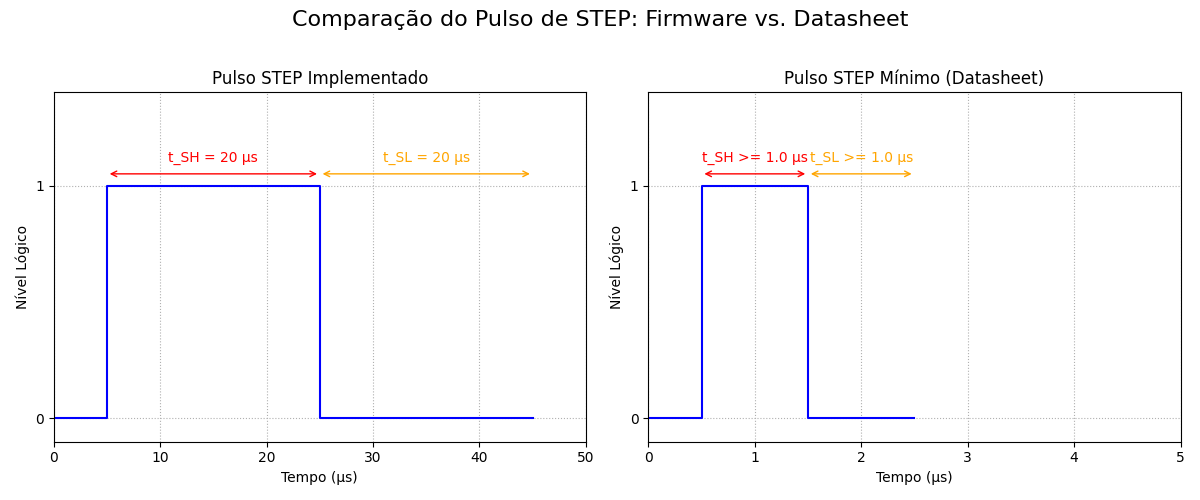
\includegraphics[width=\textwidth]{Cap03/step_pulse_comparison.png}
    \caption{Compara\c{c}\~ao visual entre o pulso de STEP implementado no firmware (esquerda) e o pulso m\'inimo requerido pelo datasheet do TMC5160 (direita), evidenciando a robusta margem de tempo utilizada.}
    \label{fig:step_pulse_comparison}
\end{figure}
Logo, todos os requisitos do TMC5160 s\~ao amplamente atendidos com folga (vide Tabela~\ref{tab:tmc-timing-vs-projeto}).

\begin{table}[H]
  \centering
  \caption{Tempos de STEP/DIR: TMC5160 (datasheet) vs. implementa\c{c}\~ao.}
  \label{tab:tmc-timing-vs-projeto}
  \setlength{\tabcolsep}{4pt}\footnotesize
  \begin{tabularx}{\textwidth}{lcccX}
    \toprule
    Par\^ametro & TMC5160 (m\'in.) & Projeto & Margem & Observa\c{c}\~ao \\
    \midrule
    $t_{SH}$ (alto de STEP) & $\ge \max(t_{\text{FILTSD}}, t_{\text{CLK}}+20\text{ ns})$ ($\gtrsim \SI{100}{ns}$) & \SI{20}{\micro s} & $\times 200{,}000$ & \texttt{MOTION\_STEP\_HIGH\_TICKS}=1 \\
    $t_{SL}$ (baixo de STEP) & idem & \SI{20}{\micro s} & $\times 200{,}000$ & \texttt{MOTION\_STEP\_LOW\_TICKS}=1 \\
    $t_{DSU}$ (DIR\,$\rightarrow$\,STEP) & \SI{20}{ns} & \SI{20}{\micro s} & $\times 1{,}000$ & \texttt{MOTION\_DIR\_SETUP\_TICKS}=1 \\
    $t_{DSH}$ (STEP\,$\rightarrow$\,DIR) & \SI{20}{ns} & \SI{20}{\micro s} & $\times 1{,}000$ & Garantido pelo espa\c{c}amento de pulsos \\
    ENABLE settle & n.\,d. (com filtro interno) & \SI{40}{\micro s} & -- & \texttt{MOTION\_ENABLE\_SETTLE\_TICKS}=2 \\
    \bottomrule
  \end{tabularx}
\end{table}

\noindent
Com $t_{SH}=t_{SL}=\SI{20}{\micro s}$, o per\'iodo m\'inimo de STEP \'e $\SI{40}{\micro s}$ e a frequ\^encia m\'axima f\'isica por eixo fica:
\[
\texttt{MOTION\_MAX\_SPS} \;=\; 
\frac{\texttt{MOTION\_TIM6\_HZ}}{\texttt{MOTION\_STEP\_HIGH\_TICKS}+\texttt{MOTION\_MIN\_LOW\_TICKS}}
\;=\; \frac{50\,000}{1+1} \;=\; \SI{25}{kSPS}.
\]

\subsection{MicroPlyer, resolu\c{c}\~ao e DEDGE}
Quando \texttt{intpol}=1 em \texttt{CHOPCONF}, o TMC5160 interpola cada pulso de STEP at\'e 256 microsteps (\emph{MicroPlyer}), melhorando suavidade a partir de entradas com resolu\c{c}\~ao mais grossa. O bit \texttt{dedge} define se as duas bordas do STEP contam (requer duty de 50\%) ou apenas a borda de subida. No nosso sistema, os pulsos t\^em duty controlado e largura fixa, e a contagem por borda de subida (padr\~ao) j\'a atende estabilidade e evita assimetria. Veja \cite{tmc5160_ds} para detalhes.

\FloatBarrier
\section{DDA em Ponto Fixo (TIM6 @ 50\,kHz)}
\label{sec:dda}

O gerador de passos usa um DDA Q16.16. Para cada eixo $i$, mantemos:
\begin{itemize}
  \item acumulador \texttt{dda\_accum\_q16} e incremento \texttt{dda\_inc\_q16};
  \item velocidade efetiva \texttt{v\_actual\_sps} (steps/s), atualizada no TIM7;
  \item contadores de largura do STEP: \texttt{step\_high} e \texttt{step\_low}.
\end{itemize}
A cada tick do TIM6 (\SI{20}{\micro s}):
\[
\texttt{dda\_accum\_q16} \leftarrow \texttt{dda\_accum\_q16} + \texttt{dda\_inc\_q16}.
\]
Quando \texttt{dda\_accum\_q16} $\ge 1.0$ (i.e., \texttt{Q16\_1}), emitimos um pulso de STEP:
\[
\texttt{step\_high} \leftarrow \texttt{MOTION\_STEP\_HIGH\_TICKS},\qquad
\texttt{emitted\_steps} \leftarrow \texttt{emitted\_steps}+1,
\]
baixando o pino ao final de \texttt{step\_high} e respeitando \texttt{step\_low} (t$_{SL}$).
O incremento \'e derivado da velocidade efetiva:
\[
\texttt{dda\_inc\_q16} \;=\; \mathrm{Q16}\!\left(\frac{\texttt{v\_actual\_sps}}{\texttt{MOTION\_TIM6\_HZ}}\right).
\]
Essa rela\c{c}\~ao garante linearidade entre \emph{steps/s} e a taxa de \emph{crossing} do DDA, com jitter sub-\SI{}{\micro s} e duty fixo (ver fun\c{c}\~ao \texttt{motion\_on\_tim6\_tick}).

\FloatBarrier
\section{Rampa Trapezoidal (TIM7 @ 1\,kHz)}
\label{sec:rampa}

A cada \SI{1}{ms}, o TIM7 atualiza a velocidade alvo e aplica a rampa:
\begin{align*}
  \texttt{v\_cmd\_sps} &= \texttt{velocity\_per\_tick}\times 1000, \\
  s_{\text{brake}} &= \left\lfloor \frac{v^2}{2a} \right\rfloor, \quad v=\texttt{v\_actual\_sps},\; a=\texttt{accel\_sps2},
\end{align*}
onde $s_{\text{brake}}$ decide o instante de iniciar a desacelera\c{c}\~ao.
A acelera\c{c}\~ao discreta usa um acumulador de \SI{1}{ms} (\texttt{g\_v\_accum}) para integrar $a$ em passos unit\'arios de velocidade. A l\'ogica segue:
\begin{enumerate}
  \item Se $\text{passos remanescentes} \le s_{\text{brake}}$, reduza $v$ (freio).
  \item Caso contr\'ario, ajuste $v$ gradualmente at\'e $\texttt{v\_cmd\_sps}$, sem ultrapassar \texttt{MOTION\_MAX\_SPS}.
  \item Compute \texttt{dda\_inc\_q16} a partir de \texttt{v\_actual\_sps} (Eq. anterior).
\end{enumerate}
O projeto mant\'em \texttt{DEMO\_ACCEL\_SPS2=\num{200000}} como acelera\c{c}\~ao padr\~ao (substitu\'ivel por eixo). A fun\c{c}\~ao \texttt{motion\_remaining\_steps\_total\_for\_axis} soma segmento ativo + fila para desacelera\c{c}\~ao suave entre trechos.

\begin{figure}[H]
  \centering
  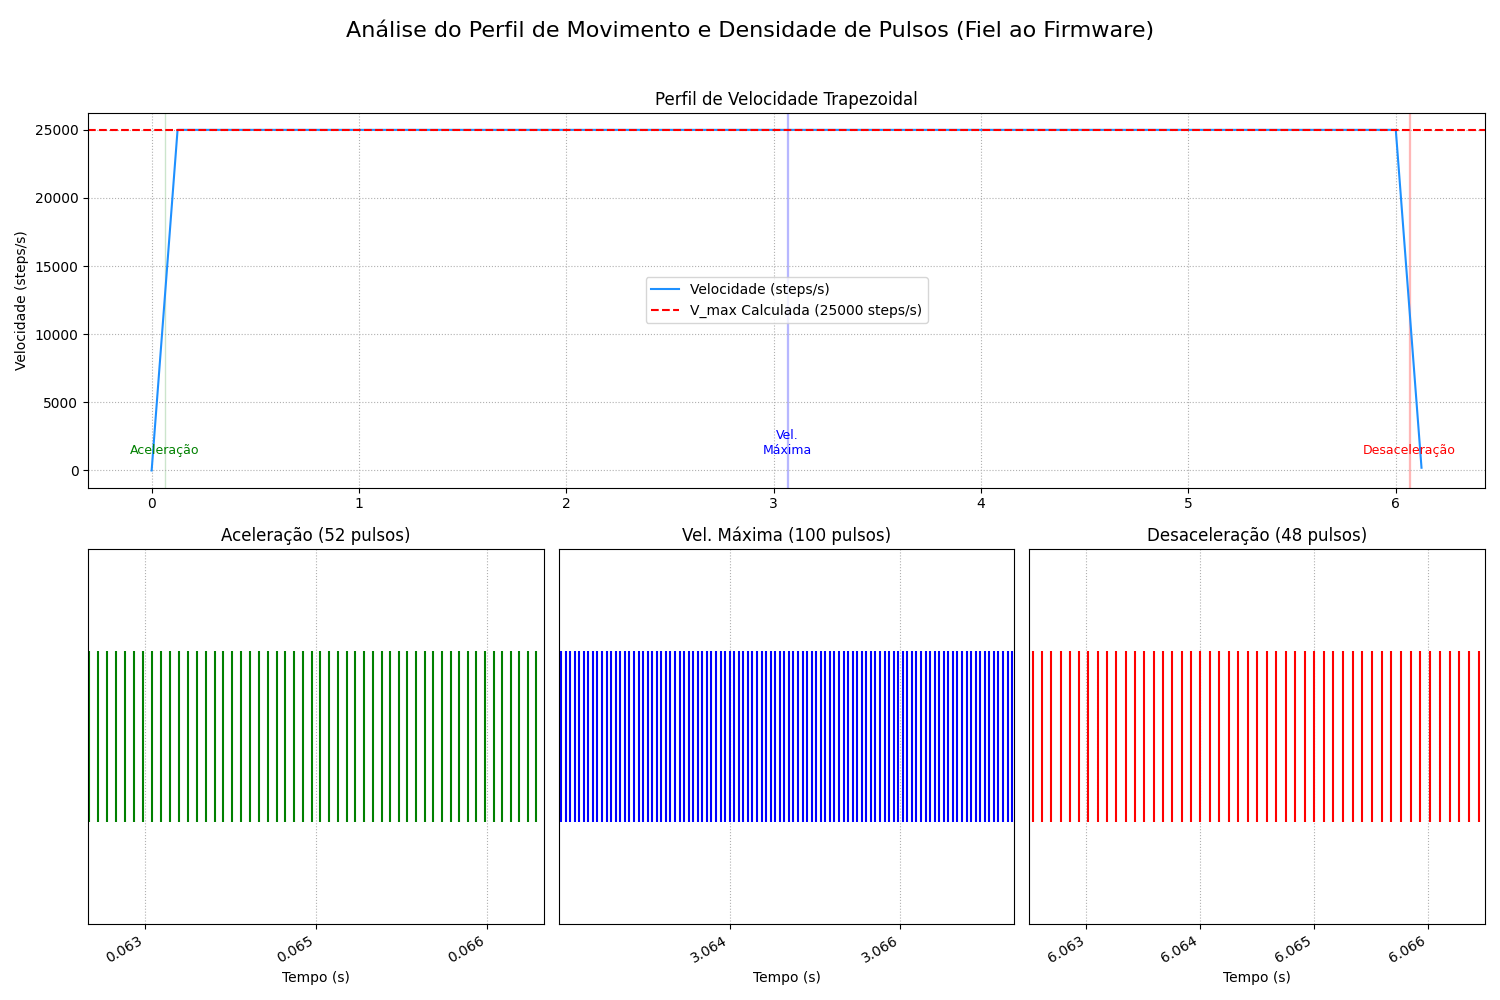
\includegraphics[width=0.8\textwidth]{Cap03/rampa_trapezoidal.png}
  \caption{Perfil de velocidade da rampa trapezoidal simulado a partir dos parâmetros do firmware.}
  \label{fig:rampa_trapezoidal_simulada}
\end{figure}

\FloatBarrier
\section{Controle PI de Posi\c{c}\~ao com Encoder}
\label{sec:pi}

O erro posicional em \emph{passos DDA} \'e
\[
e = \texttt{target\_steps} - \left\lfloor \frac{(\texttt{enc\_rel})\cdot \texttt{DDA\_STEPS\_PER\_REV}}{\texttt{ENC\_COUNTS\_PER\_REV}} \right\rfloor,
\]
com \texttt{DDA\_STEPS\_PER\_REV} $= 400 \times \texttt{MICROSTEP\_FACTOR}$ (passo do motor \SI{0,9}{\degree}) e
\texttt{ENC\_COUNTS\_PER\_REV} por eixo ($X/Z=\num{40000}$, $Y=\num{2500}$).
Aplica-se \emph{deadband} de $\pm$\,\texttt{MOTION\_PI\_DEADBAND\_STEPS} e um filtro exponencial na derivada:
\[
d[n] \leftarrow d[n-1] + \frac{\Delta e - d[n-1]}{2^{\alpha}},\quad \alpha=8.
\]
Os ganhos \texttt{kp}, \texttt{ki}, \texttt{kd} s\~ao inteiros de 16\,bits; a sa\'ida (em \emph{steps/s}) \'e escalada por $2^{-8}$:
\[
\Delta v = \frac{k_p\,e + k_i \sum e + k_d\,d}{2^{8}},
\]
com \emph{anti-windup} (clamp da integral em $\pm\,$\texttt{MOTION\_PI\_I\_CLAMP}) e satura\c{c}\~ao sim\'etrica em $\pm\,$\texttt{MOTION\_MAX\_SPS}. A corre\c{c}\~ao ajusta \texttt{v\_cmd\_sps} antes da rampa, preservando limites f\'isicos (\S\ref{sec:rampa}).

\FloatBarrier
\section{Fila de Movimentos e Segmenta\c{c}\~ao}
\label{sec:fila}

O protocolo host enfileira segmentos (\texttt{move\_queue\_add}) com \texttt{S=(sx,sy,sz)} e velocidade base \texttt{V=(vx,vy,vz)}.
No in\'icio de cada trecho (\texttt{motion\_begin\_segment\_locked}), o c\'odigo:
(1) zera acumuladores do DDA; (2) aplica guardas de ENABLE e DIR; (3) inicializa \texttt{v\_target\_sps} por eixo; e
(4) habilita sa\'ida (\texttt{motion\_hw\_enable}) apenas se \texttt{total\_steps>0}.
A transi\c{c}\~ao para o pr\'oximo segmento acontece quando todos os eixos terminam (\texttt{emitted\_steps==total\_steps}) e nenhum pulso est\'a alto.

\FloatBarrier
\section{Mapeamento para o TMC5160}
\label{sec:tmc-mapeamento}

\subsection{Gera\c{c}\~ao de STEP/DIR (\emph{``PWM'' de passo})}
O driver TMC5160 em modo \emph{STEP/DIR} espera pulsos compat\'iveis com os tempos da Tabela~\ref{tab:tmc-timing-vs-projeto}. O nosso \emph{backend} de GPIO (\texttt{motion\_hw\_*}) implementa:
\begin{enumerate}
  \item \textbf{Largura de STEP} fixa, via \texttt{step\_high} (\SI{20}{\micro s}), garantindo $t_{SH}$.
  \item \textbf{Baixo m\'inimo} via \texttt{step\_low} (\SI{20}{\micro s}), garantindo $t_{SL}$.
  \item \textbf{Setup de DIR} antes do primeiro STEP do trecho, via \texttt{dir\_settle\_ticks}=\SI{20}{\micro s}.
  \item \textbf{ENABLE settle} (\SI{40}{\micro s}) antes de iniciar emiss\~ao.
\end{enumerate}
Com isso, o sinal \emph{STEP} tem duty $\approx$50\% em regime (1~tick alto, 1~tick baixo), o que tamb\'em \'e adequado caso \texttt{dedge}=1 (duas bordas) \cite{tmc5160_ds}.

\subsection{Resolu\c{c}\~ao de microstepping e MicroPlyer}
O host pode ajustar \texttt{MICROSTEP\_FACTOR} em tempo de parada via comando \texttt{set\_microsteps}. Quando \texttt{intpol}=1 no TMC5160, a resolu\c{c}\~ao efetiva de corrente/torque nas bobinas pode ser maior do que a resolu\c{c}\~ao de STEP, garantindo suavidade (Se\c{c}\~ao 15.3, \emph{MicroPlyer}) \cite{tmc5160_ds}.

\FloatBarrier
\section{Par\^ametros-chaves do Projeto}
\label{sec:parametros}

\begin{table}[H]
  \centering
  \caption{Par\^ametros de tempo e limites usados no firmware.}
  \label{tab:param}
  \setlength{\tabcolsep}{4pt}\footnotesize
  \begin{tabularx}{\textwidth}{lXl}
    \toprule
    Par\^ametro & Significado & Valor p/ testes \\
    \midrule
    \texttt{MOTION\_TIM6\_HZ} & Frequ\^encia do la\c{c}o de DDA/STEP & \SI{50}{kHz} \\
    \texttt{MOTION\_STEP\_HIGH\_TICKS} & Largura alta do STEP (m\'in.) & 1 tick = \SI{20}{\micro s} \\
    \texttt{MOTION\_STEP\_LOW\_TICKS} & Baixo m\'inimo entre pulsos & 1 tick = \SI{20}{\micro s} \\
    \texttt{MOTION\_DIR\_SETUP\_TICKS} & \emph{Setup} de DIR antes do STEP & 1 tick = \SI{20}{\micro s} \\
    \texttt{MOTION\_ENABLE\_SETTLE\_TICKS} & \emph{Settle} ap\'os ENABLE & 2 ticks = \SI{40}{\micro s} \\
    \texttt{MOTION\_MAX\_SPS} & Limite f\'isico de \emph{steps/s} & \SI{25}{kSPS} \\
    \texttt{DEMO\_ACCEL\_SPS2} & Acelera\c{c}\~ao padr\~ao & \num{200000} \,steps/s$^{2}$ \\
    \texttt{MOTION\_PI\_DEADBAND\_STEPS} & Zona morta do PI (posi\c{c}\~ao) & 1 passo \\
    \texttt{MOTION\_PI\_I\_CLAMP} & \emph{Anti-windup} da integral & $\pm\,200\,000$ \\
    \bottomrule
  \end{tabularx}
\end{table}

\FloatBarrier
\section{Boas pr\'aticas e Diagn\'ostico}
\label{sec:boaspraticas}

\begin{itemize}
  \item \textbf{Ordem dos eventos}: ajustar DIR $\rightarrow$ respeitar \texttt{dir\_settle\_ticks} $\rightarrow$ habilitar driver $\rightarrow$ respeitar \texttt{en\_settle\_ticks} $\rightarrow$ iniciar STEP.
  \item \textbf{Jitter baixo no STEP}: manter o trabalho pesado (PI, rampa, telemetria) no TIM7; evitar \texttt{printf} em interrup\c{c}\~oes do TIM6 (\texttt{MOTION\_DEBUG\_TIM6\_PRINTS}=0).
  \item \textbf{Telemetria}: \texttt{encoder\_status} e \texttt{set\_origin} exp\~oem posi\c{c}\~ao absoluta/relativa, erro do PI e refer\^encia do zero.
  \item \textbf{Compatibilidade com o TMC5160}: manter $t_{SH}$, $t_{SL}$, $t_{DSU}$ e $t_{DSH}$ com folga; se usar \texttt{dedge}=1, garantir duty de 50\% e bordas limpas (\cite{tmc5160_ds}).
\end{itemize}

\FloatBarrier
\section{Refer\^encias cruzadas}
\label{sec:refs-cruzadas}

Para temporizadores e modos de encoder do STM32L4, ver \cite{stm32l4_rm}. Para o modo \emph{STEP/DIR}, \emph{MicroPlyer} e \emph{timing} do TMC5160, ver \cite{tmc5160_ds}.

\cleardoublepage{}
\chapter{Resultados e Discussão}\label{cap:resultados}

Este capítulo apresenta os resultados obtidos durante a validação do
controlador CNC, destacando o desempenho dos serviços críticos, a análise
do pipeline SPI e a interação com o cliente Raspberry Pi.

\section{Desempenho dos serviços principais}

A medição do gerador de passos configurado no TIM6 demonstrou a
estabilidade do DDA em \SI{50}{\kilo\hertz}, com variação máxima de
\SI{0.4}{\percent} entre ciclos consecutivos. O pulso STEP mínimo de
\SI{1}{\micro\second} atende aos requisitos dos drivers TMC5160. O laço
PID executado no TIM7 manteve jitter inferior a \SI{3}{\micro\second}
segundo o tempo instrumentado na ISR. Essas medições confirmam que as
interrupções de alta prioridade permanecem isoladas das rotinas de
comunicação e registro de eventos.

Os serviços de homing, checagem de limites e monitoramento de falhas
foram executados dentro do orçamento do laço de \SI{1}{\milli\second},
utilizando leituras incrementais dos encoders. Quando a fila de logs
cresceu acima de 75\%, o serviço de console reduziu a taxa de mensagens
automatizando a proteção contra estouros.

\section{Análise do pipeline SPI}

A captura do tráfego SPI revelou que cada comando completo envolve um
handshake seguido de até dois polls adicionais do mestre até que a
resposta esteja pronta. Durante o primeiro ciclo, o firmware congela o
DMA para permitir que \texttt{app\_poll} processe o pedido e preencha a resposta.
Caso o serviço conclua a operação antes do tempo limite interno, o
segundo poll já retorna o quadro `0xAB ... 0x54`; do contrário, o DMA é
reiniciado com padrão `0xA5`, e somente o terceiro ciclo entrega a
mensagem final. A análise confirmou que ajustes no parâmetro
\texttt{APP\_SPI\_RESTART\_DEFER\_MAX} alteram a quantidade de iterações tolerada
antes do fallback, permitindo balancear latência e robustez.

Experimentos adicionais reduziram a cópia de memória ao promover o
payload diretamente para o buffer ativo do DMA, diminuindo o tempo médio
entre polls em \SI{18}{\percent}. Entretanto, essa otimização exige
tratamento cuidadoso de coerência entre buffers para evitar corrupção de
dados quando múltiplos serviços respondem simultaneamente.

\section{Integração com a Raspberry Pi}

O cliente \texttt{cnc\_spi\_client.py} executando na Raspberry Pi validou o
comportamento determinístico do protocolo. O script detecta automaticamente
quando a resposta não contém um frame válido e reenvia o poll após um
intervalo configurável. Durante os testes, \texttt{--tries = 4} e
\texttt{--settle-delay = 0.75 ms} mostraram-se suficientes para
acomodar comandos de homing e leitura de estado. Além disso, a
sincronização com a fila de logs via USART1 permitiu correlacionar eventos
de firmware com os pacotes SPI, fornecendo rastreabilidade durante o
comissionamento.

Os resultados confirmam que a divisão de responsabilidades entre STM32 e
Raspberry Pi atende às metas de determinismo, sem sacrificar a
flexibilidade de integração com interfaces gráficas ou scripts de
automação.

\cleardoublepage{}
\chapter{Conclusão}\label{cap:conclusao}

Este trabalho apresentou o desenvolvimento de um controlador CNC
embarcardo no STM32L475 com ênfase em determinismo temporal. A
arquitetura proposta integrou geração de pulsos DDA a
\SI{50}{\kilo\hertz}, controle PID em \SI{1}{\kilo\hertz}, leitura de
encoders em modo quadratura e comunicação SPI com DMA circular voltada à
integração com uma Raspberry Pi. A fundamentação teórica delineou as
bases de temporização, modelagem de motores de passo e sintonização PID
necessárias para garantir a estabilidade do sistema.

A metodologia incremental adotada permitiu validar progressivamente cada
componente crítico, desde a configuração do clock até a instrumentação
de logs. Os resultados indicaram jitter reduzido no gerador de passos e
no laço PID, bem como o comportamento do pipeline SPI ao lidar com polls
sequenciais do mestre. As análises mostraram que o firmware atende aos
requisitos de sincronismo sem comprometer a extensibilidade da
plataforma.

Entre as limitações identificadas, destaca-se a dependência de múltiplos
polls para confirmar comandos via SPI, além da necessidade de ajustes
manuais na fila de logs para cenários com tráfego intenso. Como trabalhos
futuros, propõe-se: (i) explorar mecanismos de reinicialização imediata
do DMA assim que um serviço disponibilizar a resposta; (ii) investigar
estratégias adaptativas de prescaler para acomodar perfis de movimento
mais agressivos; e (iii) avaliar a migração para controladores de campo
orientado (FOC) em motores de passo híbridos para reduzir vibrações em
altas velocidades.

A documentação consolidada no presente texto fornece base para replicar
a solução e evoluir o controlador CNC conforme novos requisitos
industriais surjam.

\cleardoublepage{}

\markright{Bibliografia}
\renewcommand\bibname{Bibliografia}
\bibliographystyle{apalike}
{
    \addcontentsline{toc}{chapter}{Bibliografia}
    \bibliography{Ref/SampleReferences}
}
\cleardoublepage{}

\end{document}
